% Proposta F (12/11/2026, pedido do autor): a E ficou simples demais. Meio-termo
% entre a C e a E. Da E: setas com o nome do que levam, sem legenda e sem fórmula.
% Da C: o filtro como pergunta, o veto e o ajuste da posição como etapas. O losango
% fica no ramo do GARCH, então só a volatilidade entra nele (era o defeito da C).
% O sinal do ARIMA desce até o ajuste e só passa quando o filtro libera.
% Mesmo estilo das fig05/fig06. Fora do TG até o autor decidir.
\documentclass[11pt,border=2pt]{standalone}
\usepackage[T1]{fontenc}
\usepackage[utf8]{inputenc}
\usepackage{mathptmx}
\usepackage{tikz}
\usetikzlibrary{arrows.meta,positioning,calc,shapes.geometric}
\tikzset{
  seta/.style={-{Stealth[length=2.2mm]}, semithick},
  caixa/.style={rectangle, draw, semithick, fill=gray!10, rounded corners=2pt,
                align=center, minimum width=42mm, minimum height=10mm, font=\small},
  dado/.style={trapezium, trapezium left angle=75, trapezium right angle=105, draw,
               semithick, fill=white, align=center, minimum height=9mm, font=\small,
               trapezium stretches body},
  decisao/.style={diamond, draw, semithick, fill=white, aspect=2.2, align=center,
                  inner sep=0.5pt, font=\small},
  rotulo/.style={font=\footnotesize, align=center, fill=white, inner sep=1.5pt},
  pergunta/.style={font=\small\itshape, align=center},
}
\begin{document}
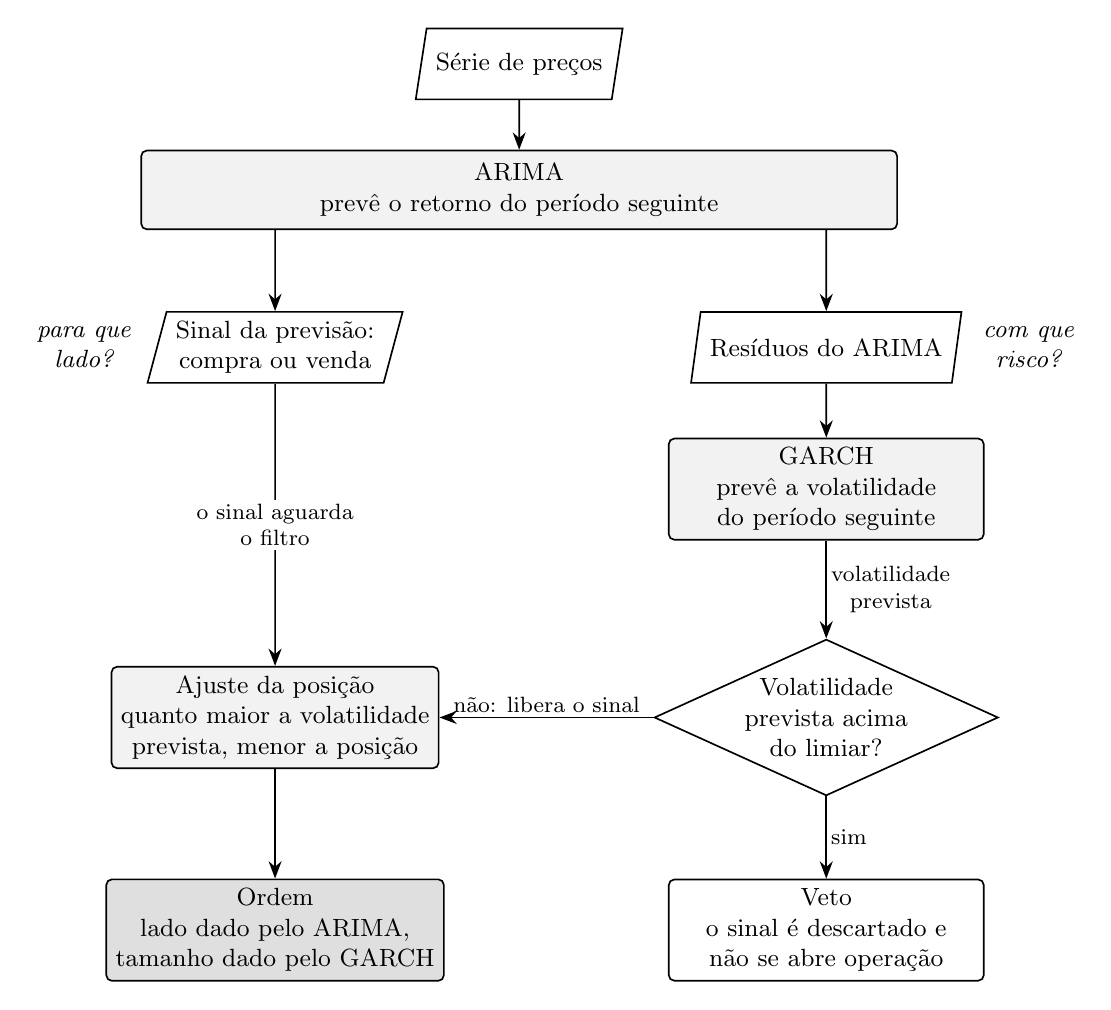
\begin{tikzpicture}
  \def\xa{-3.1}  % ramo da direção
  \def\xg{3.9}   % ramo do risco
  \node[dado] (ent) at (0,0) {Série de preços};
  \node[caixa, minimum width=96mm] (arima) at (0,-1.6) {ARIMA\\prevê o retorno do período seguinte};

  % ramo da direção
  \node[dado] (sinal) at (\xa,-3.6) {Sinal da previsão:\\compra ou venda};
  \node[caixa, minimum width=40mm] (ajuste) at (\xa,-8.3)
    {Ajuste da posição\\quanto maior a volatilidade\\prevista, menor a posição};
  \node[caixa, fill=gray!25, minimum width=40mm] (ordem) at (\xa,-11.0)
    {Ordem\\lado dado pelo ARIMA,\\tamanho dado pelo GARCH};

  % ramo do risco
  \node[dado] (res) at (\xg,-3.6) {Resíduos do ARIMA};
  \node[caixa, minimum width=40mm] (garch) at (\xg,-5.4) {GARCH\\prevê a volatilidade\\do período seguinte};
  \node[decisao] (filtro) at (\xg,-8.3) {Volatilidade\\prevista acima\\do limiar?};
  \node[caixa, fill=white, minimum width=40mm] (veto) at (\xg,-11.0)
    {Veto\\o sinal é descartado e\\não se abre operação};

  \draw[seta] (ent) -- (arima);
  \draw[seta] (arima.south -| sinal) -- (sinal);
  \draw[seta] (arima.south -| res) -- (res);
  \draw[seta] (res) -- (garch);
  \draw[seta] (garch) -- node[rotulo, right, fill=none]{volatilidade\\prevista} (filtro);
  \draw[seta] (sinal) -- node[rotulo]{o sinal aguarda\\o filtro} (ajuste);
  \draw[seta] (filtro) -- node[rotulo, above, fill=none]{não: libera o sinal} (ajuste);
  \draw[seta] (filtro) -- node[rotulo, right, fill=none]{sim} (veto);
  \draw[seta] (ajuste) -- (ordem);

  \node[pergunta, anchor=east] at ([xshift=-2mm]sinal.west) {para que\\lado?};
  \node[pergunta, anchor=west] at ([xshift=2mm]res.east) {com que\\risco?};
\end{tikzpicture}
\end{document}
